Charakterystyki dynamiczne sensorów temperatury wyznacza się na podstawie ich stałej czasowej.
Wartość tę określa czas, jakiego sensor potrzebuje, aby jego odpowiedź dynamiczna osiągnęła 63.2\%
stabilizacji po gwałtownej zmianie temperatury jego otoczenia. Przykładową odpowiedź
skokową~z~widoczną charakterystyką dynamiczą przedstawia rysunek \ref{img:transfer-rtd}
\cite{gawedzki2010}. Stałą czasową sensorów termorezystancyjnych oraz termoelektrycznych można
wyznaczyć korzystając~z~zależności:

\begin{equation}
  \tau = \frac{x}{K}\cdot\rho\cdot l\cdot C
\end{equation}

\begin{eqparams}
  x & grubość elementu (termorezystora, termoogniwa), \\
  l & długość elementu, \\
  K & przewodność termiczna, charakterystyczna dla materiału,\\
  \rho & gęstość materiału, \\
  C & pojemność cieplna, charakterystyki dla materiału
\end{eqparams}

\begin{figure}[!htbp]
  \centering
  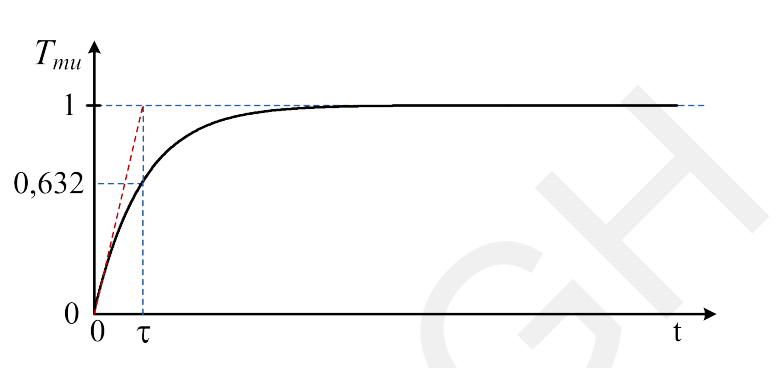
\includegraphics[width=0.7\textwidth]{sensor-theory/transfer-rtd}
  \caption{\label{img:transfer-rtd}Przykładowe odpowiedzi skokowe sensorów temperatury.}
\end{figure}